% ------------------------------------------------------------
% File: figures/fig-iteration-2-gate-popout.tex
% Iteration 2 gate formation microscopy callout: x20 image -> x100 image
% ------------------------------------------------------------

\begin{figure}[htbp]
  \centering
  \begin{tikzpicture}[
    callout/.style={dashed, line width=1.75 pt},
    connector/.style={dashed, line width=1pt, opacity=0.85}
  ]
    % Manual adjustment controls:
    % - Source box on the x20 image. Fractions are measured from the top-left
    %   of the x20 image. Move these to place the box over the completed gate.
    \def\xTwentyBoxLeft{0.35}
    \def\xTwentyBoxRight{0.59}
    \def\xTwentyBoxTop{0.18}
    \def\xTwentyBoxBottom{0.42}

    \node[anchor=north west, inner sep=0pt] (xTwenty) at (0,0) {
      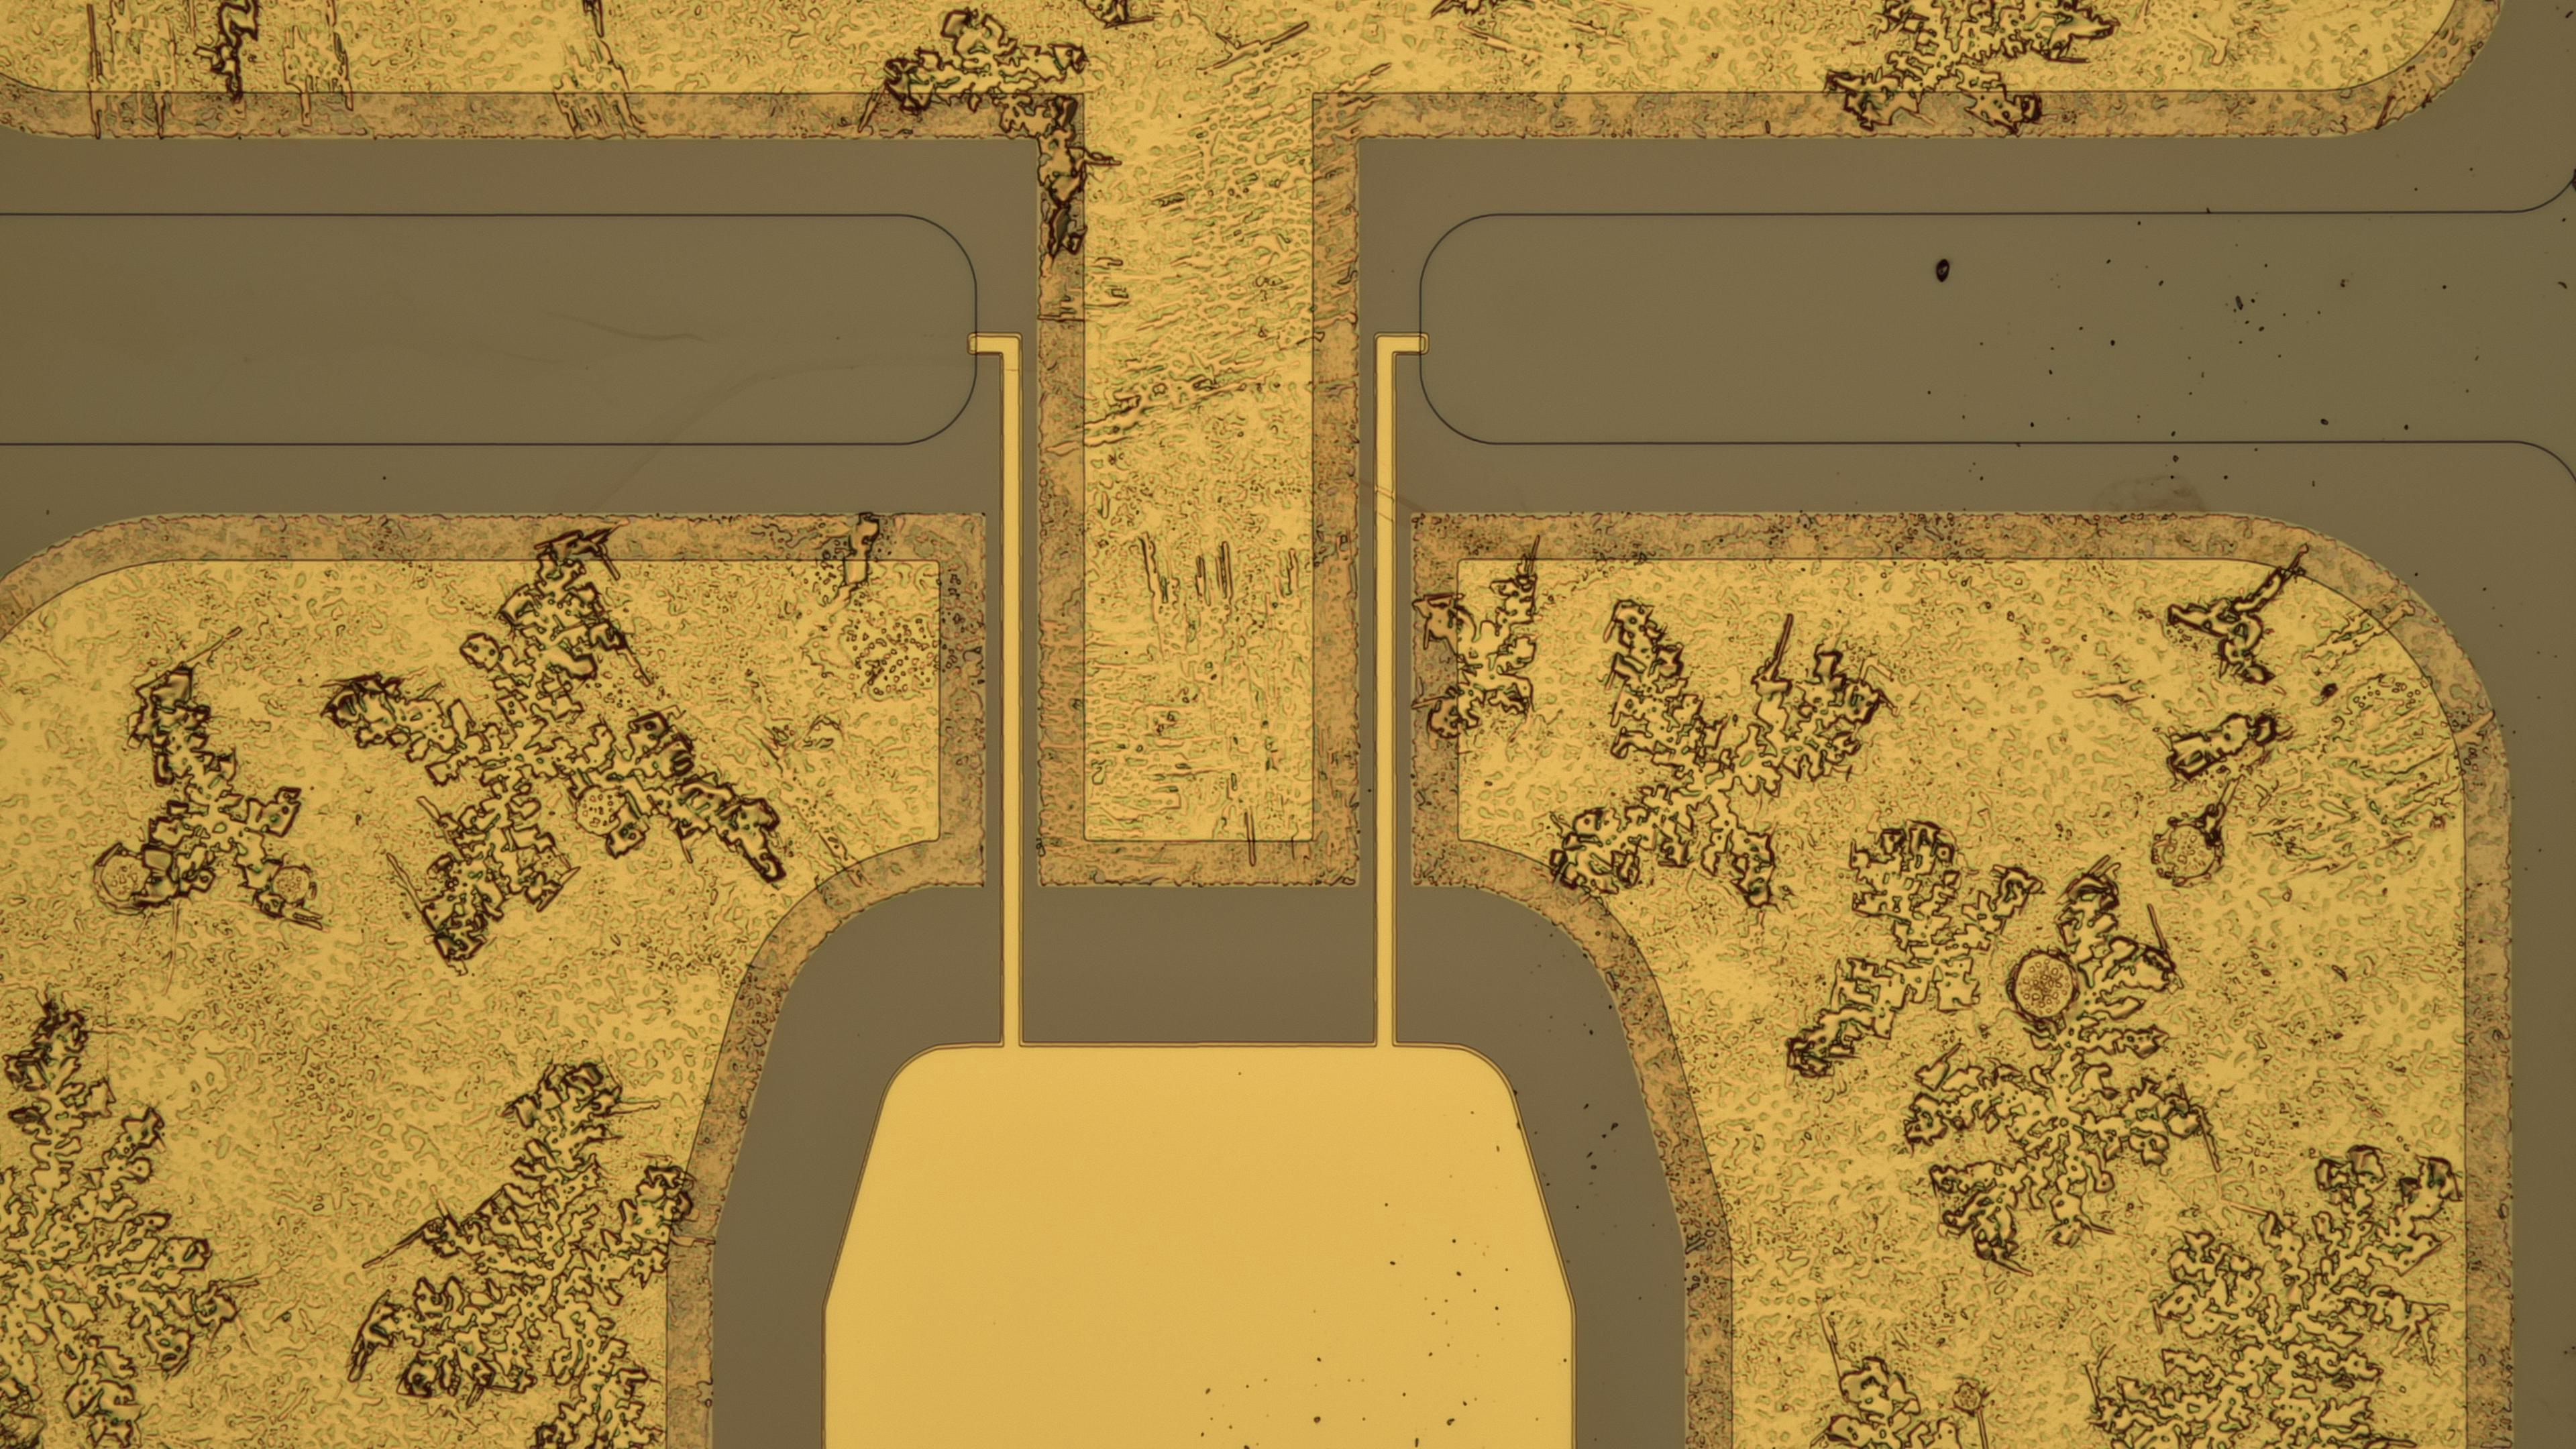
\includegraphics[width=0.475\linewidth]{figures/fabrication_images/enhancement_mode_images/iteration2/gate-formation.jpg}
    };

    \node[anchor=north west, inner sep=0pt] (xHundred) at ($(xTwenty.north east)+(0.04\linewidth,0)$) {
      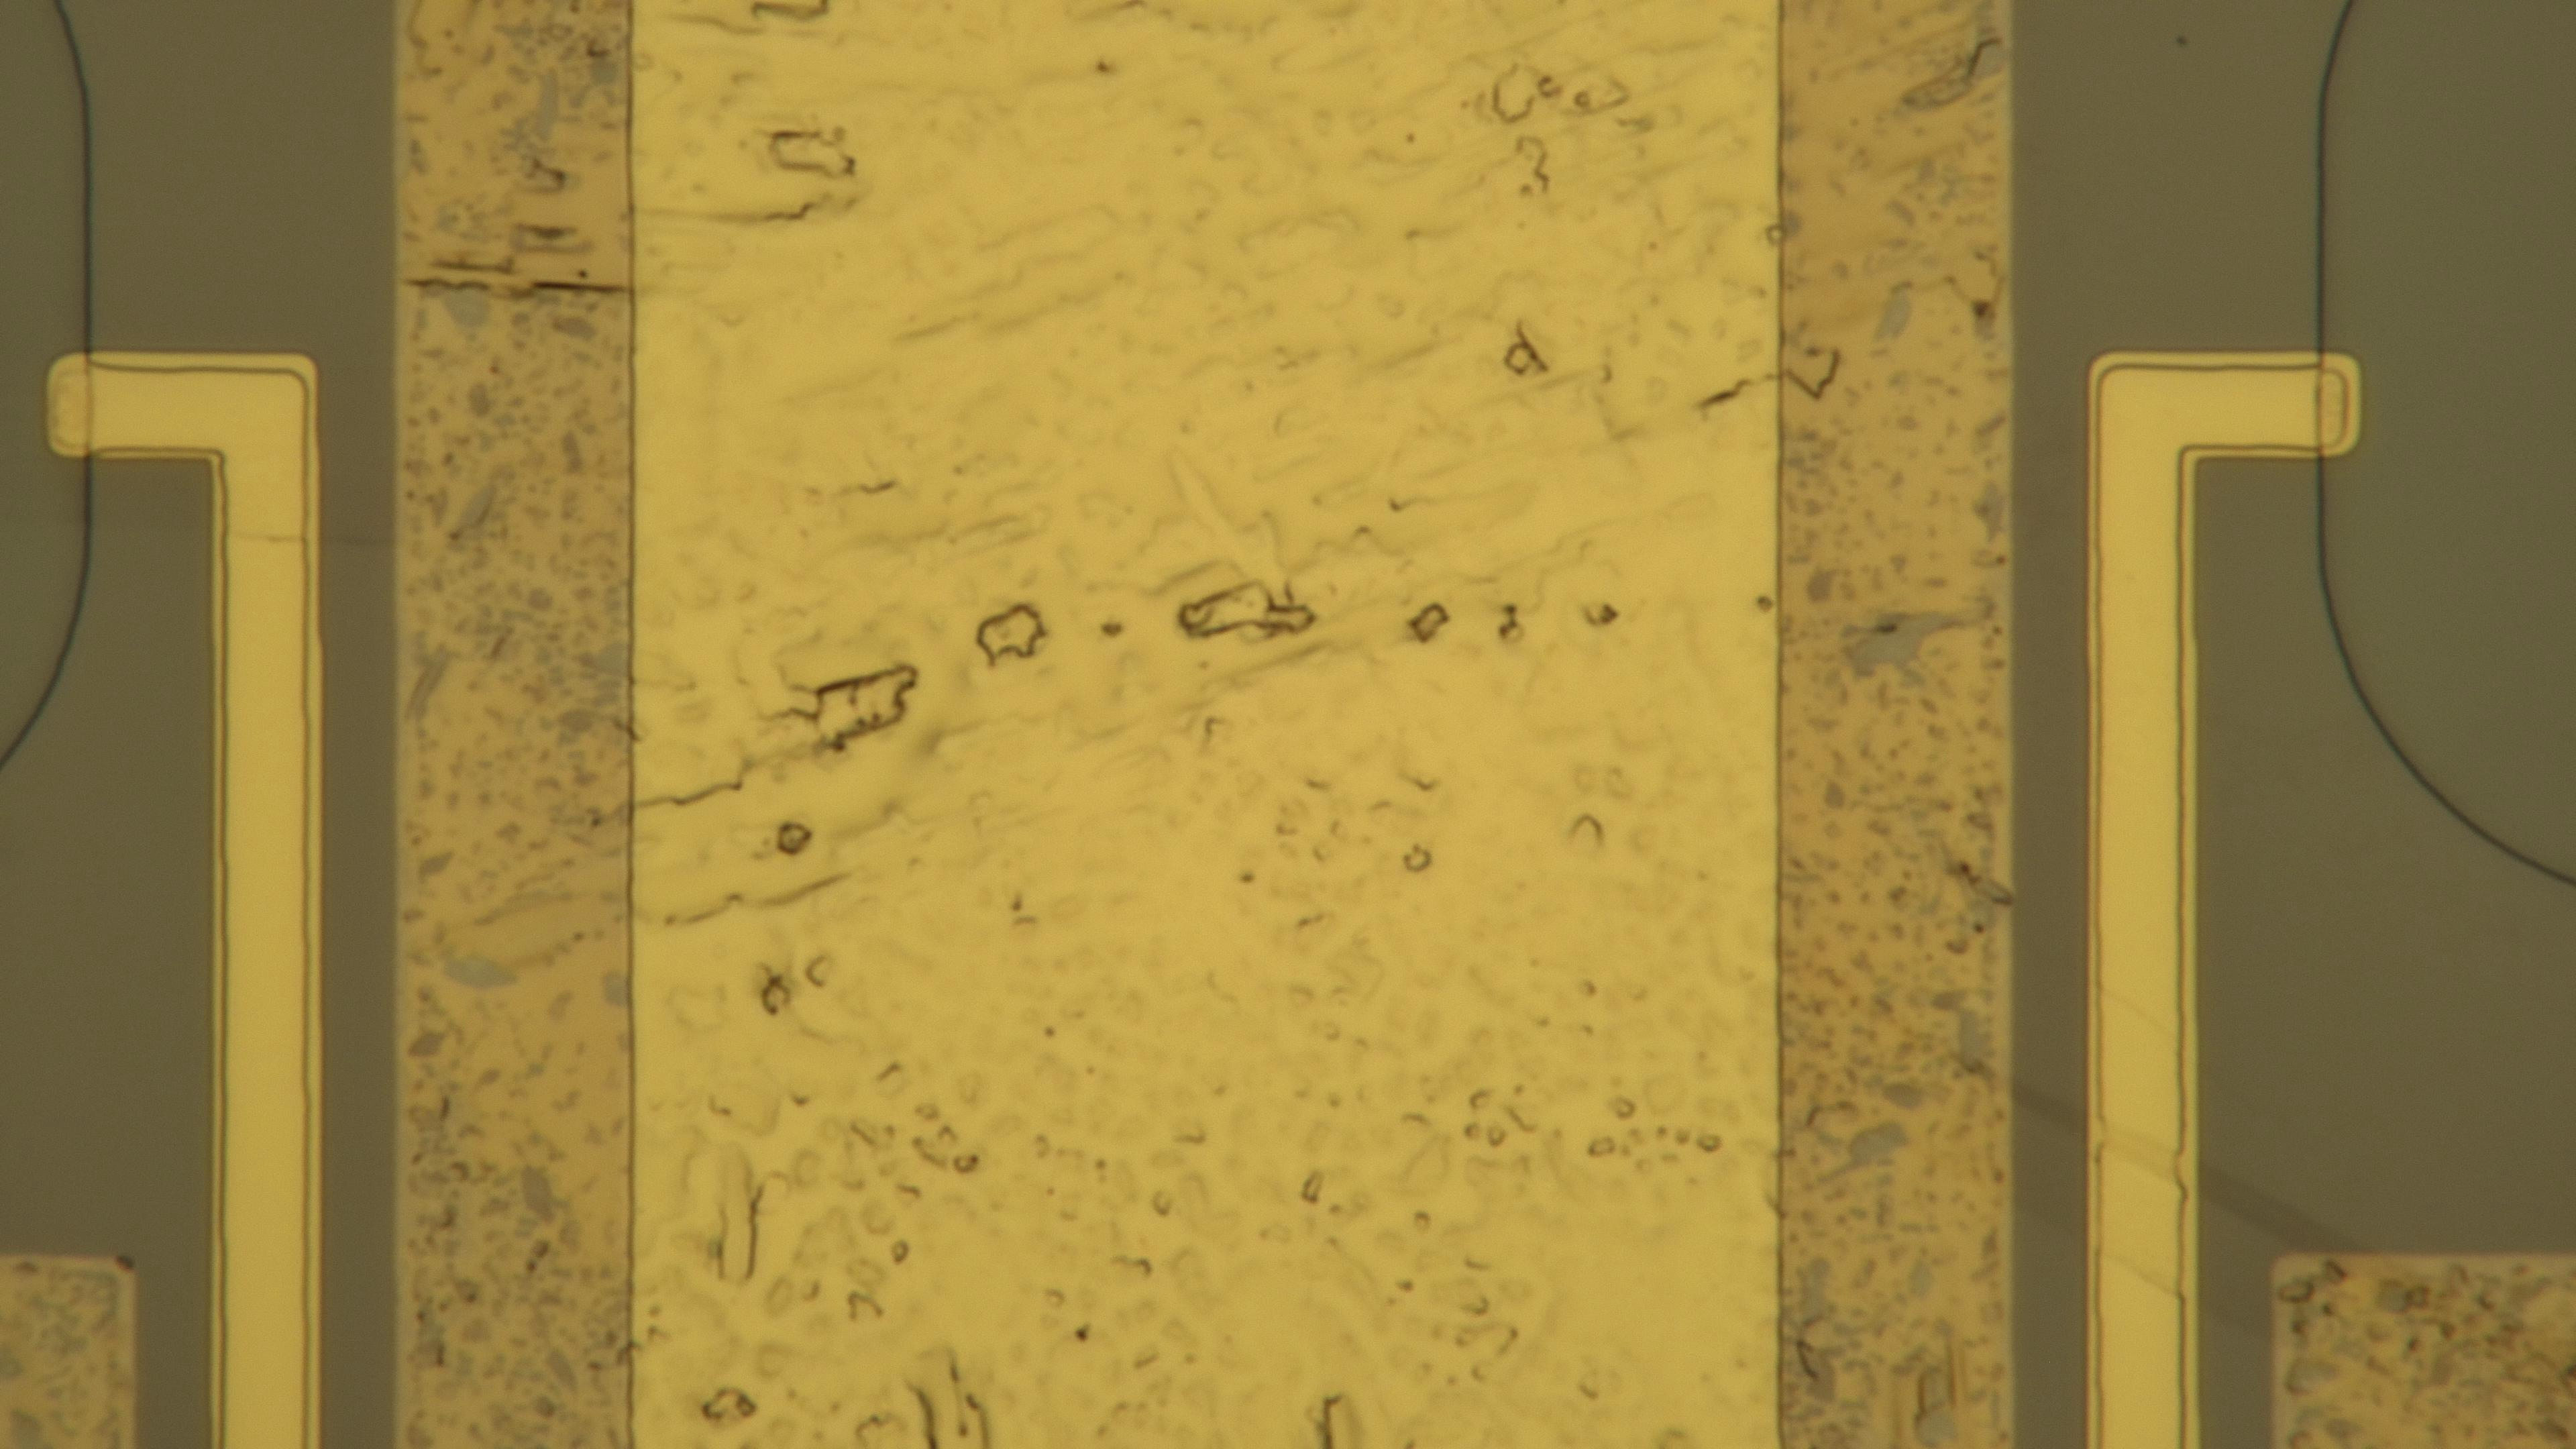
\includegraphics[width=0.475\linewidth]{figures/fabrication_images/enhancement_mode_images/iteration2/gate_formation_x100.jpg}
    };

    % Adjustable source callout on the x20 image.
    \path let \p1=(xTwenty.north west), \p2=(xTwenty.south east) in
      coordinate (xTwentyBoxNW) at ({\x1+\xTwentyBoxLeft*(\x2-\x1)}, {\y1+\xTwentyBoxTop*(\y2-\y1)})
      coordinate (xTwentyBoxNE) at ({\x1+\xTwentyBoxRight*(\x2-\x1)}, {\y1+\xTwentyBoxTop*(\y2-\y1)})
      coordinate (xTwentyBoxSW) at ({\x1+\xTwentyBoxLeft*(\x2-\x1)}, {\y1+\xTwentyBoxBottom*(\y2-\y1)})
      coordinate (xTwentyBoxSE) at ({\x1+\xTwentyBoxRight*(\x2-\x1)}, {\y1+\xTwentyBoxBottom*(\y2-\y1)});

    \draw[callout, red!75!black]
      (xTwentyBoxNW) rectangle (xTwentyBoxSE);

    % Destination border around the full x100 image.
    \coordinate (xHundredBoxNW) at ($(xHundred.north west)+(0.03,-0.03)$);
    \coordinate (xHundredBoxNE) at ($(xHundred.north east)+(-0.03,-0.03)$);
    \coordinate (xHundredBoxSW) at ($(xHundred.south west)+(0.03,0.03)$);
    \coordinate (xHundredBoxSE) at ($(xHundred.south east)+(-0.03,0.03)$);

    \draw[connector, red!75!black]
      (xTwentyBoxNW) -- (xHundredBoxNW);
    \draw[connector, red!75!black]
      (xTwentyBoxNE) -- (xHundredBoxNE);
    \draw[connector, red!75!black]
      (xTwentyBoxSW) -- (xHundredBoxSW);
    \draw[connector, red!75!black]
      (xTwentyBoxSE) -- (xHundredBoxSE);

    % Redraw the x100 image so connector lines sit beneath the destination.
    \node[anchor=north west, inner sep=0pt] at (xHundred.north west) {
      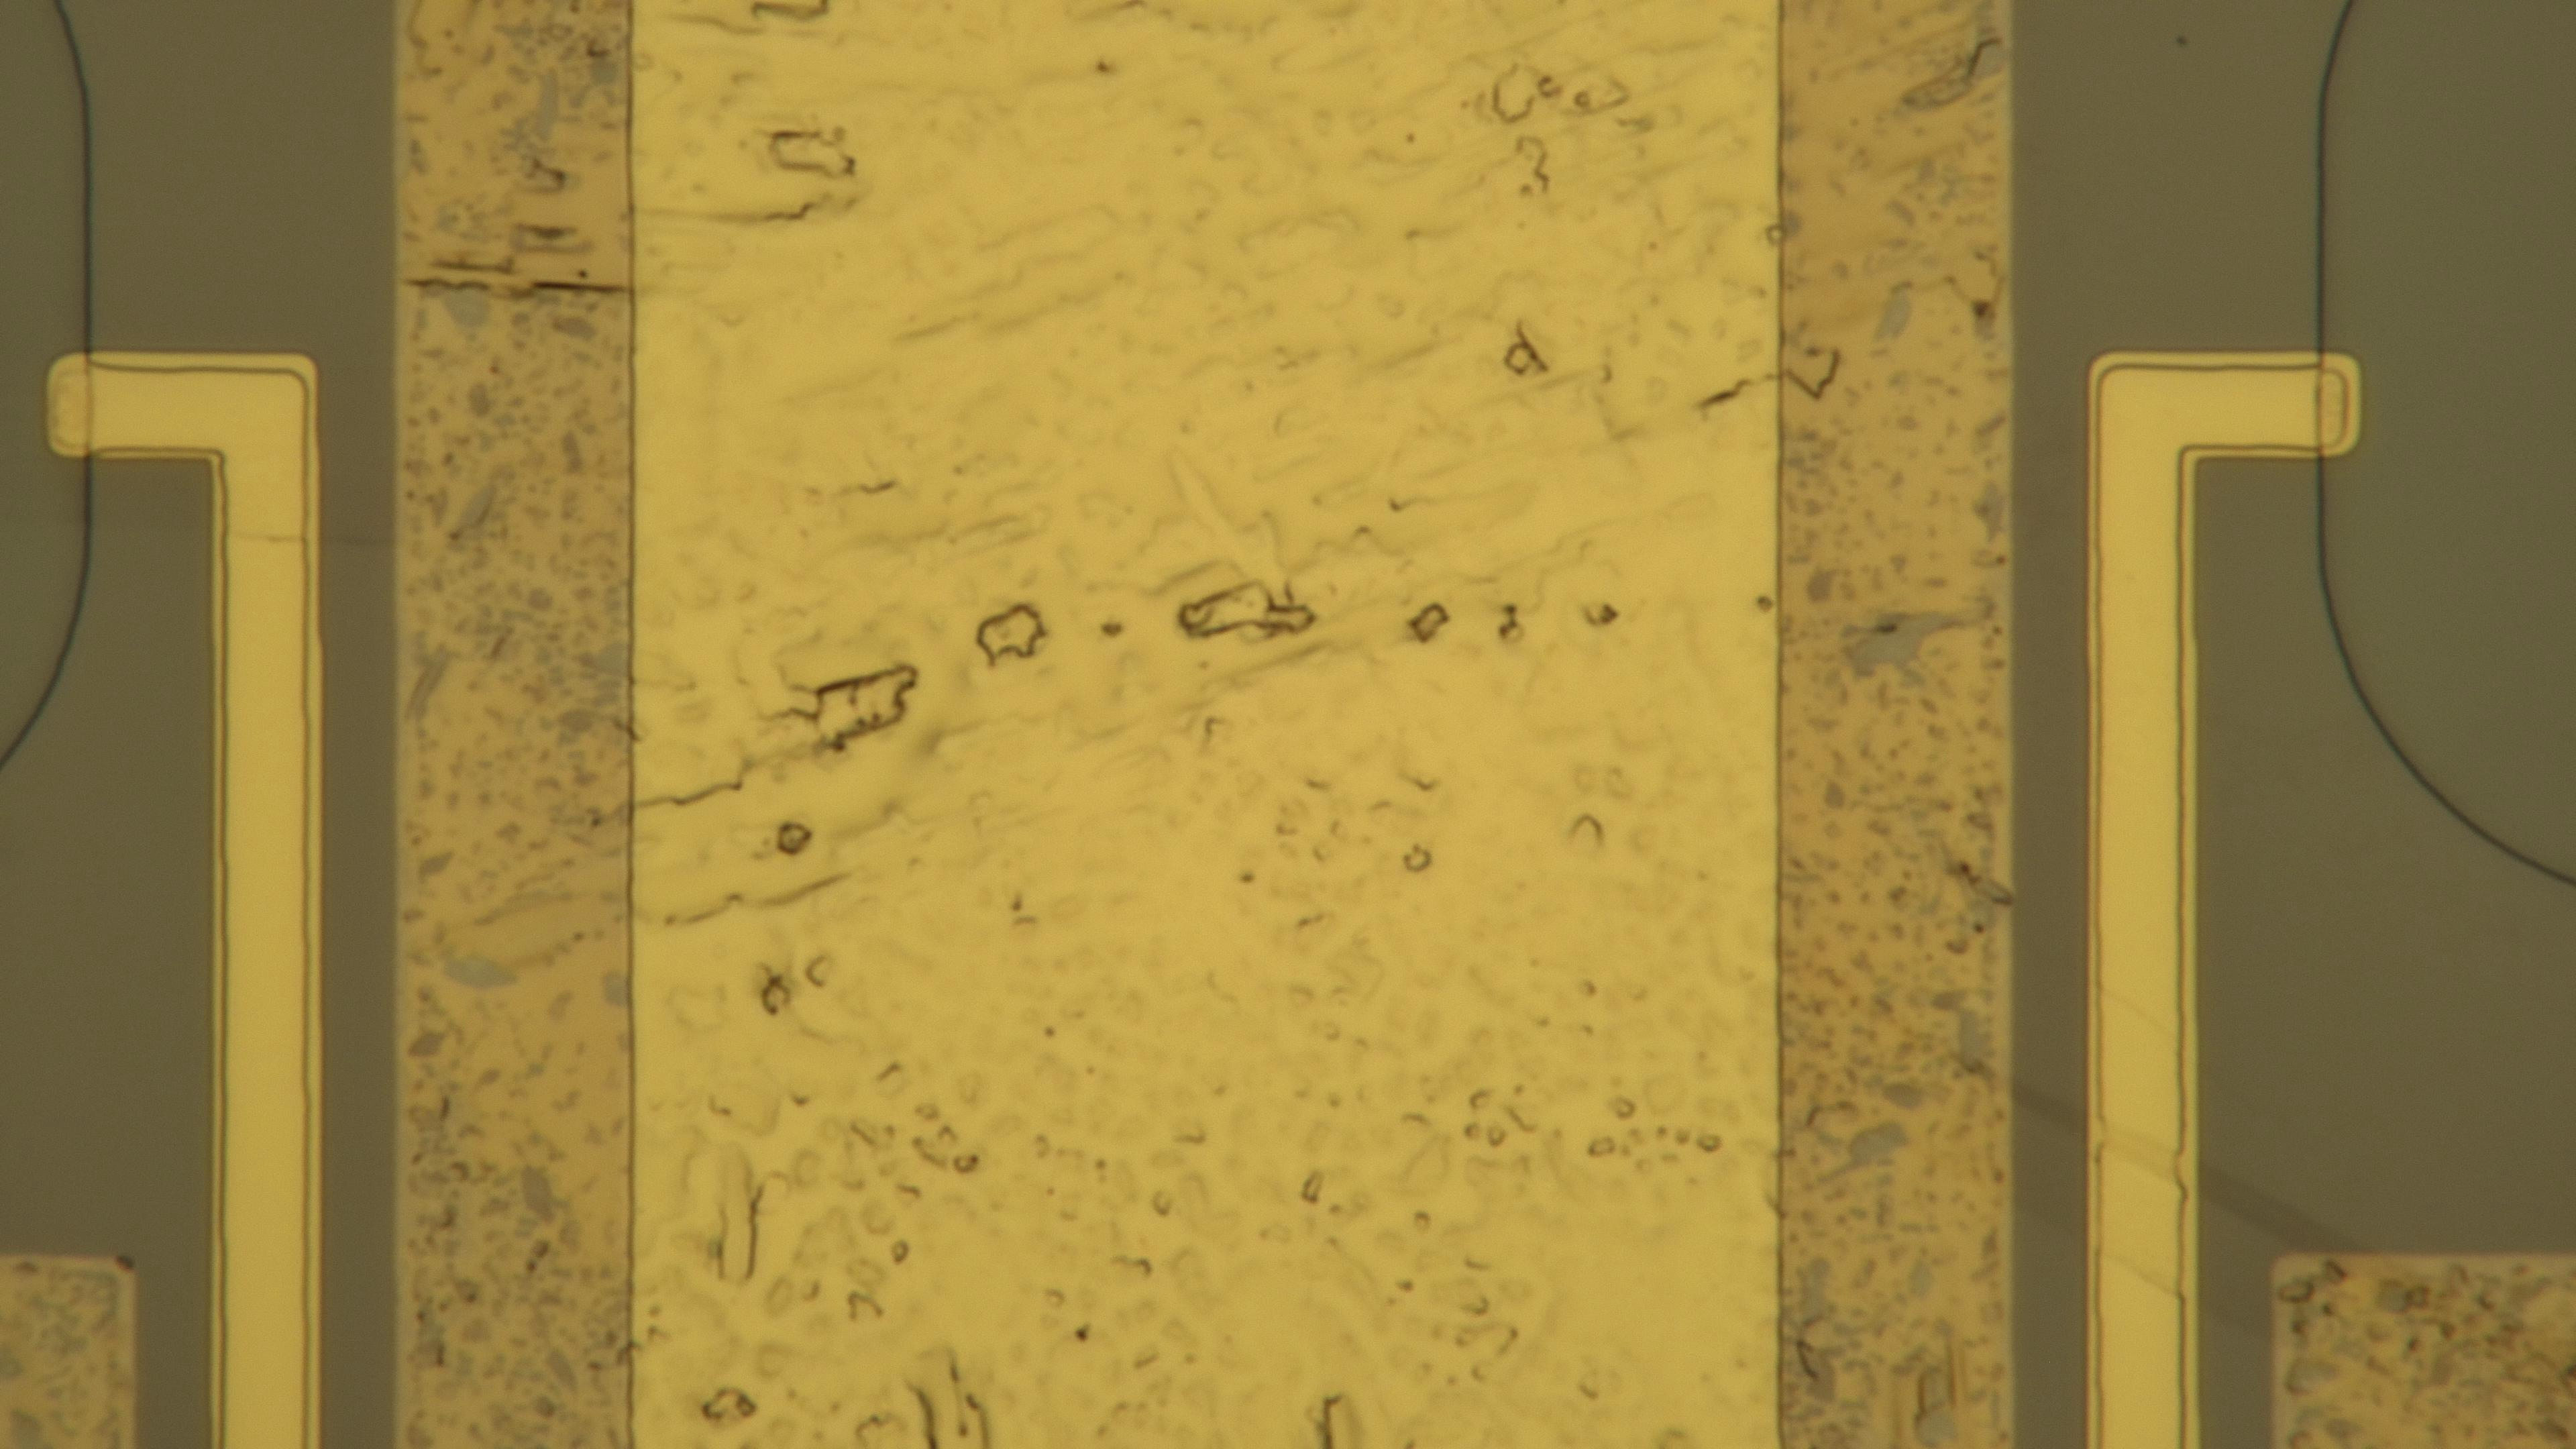
\includegraphics[width=0.475\linewidth]{figures/fabrication_images/enhancement_mode_images/iteration2/gate_formation_x100.jpg}
    };

    \draw[callout, red!75!black]
      (xHundredBoxNW) rectangle (xHundredBoxSE);
  \end{tikzpicture}

  \vspace{3pt}
  \caption{Optical microscopy of Iteration 2 gate formation.}
  \label{fig:iteration2-gate-popout}
\end{figure}
